\section{GPU and CPU performance}
\label{sec:perf}

\noindent\fbox{\parbox{\dimexpr\textwidth-2\fboxsep-2\fboxrule\relax}{%
\textbf{Interim version, 2 November 2026.} Two single-core runs of the
extruded cases (Brantley--Larsen SDP3 with 16 layers, C5G7 SDP3 with 8 layers)
and the two concurrency controls of the extruded jobs are still running and
are expected to finish by the evening of 3 November. This section quotes
projections for them, and for the extruded GMRES cases that will not be
measured on one core; it will be updated with the measurements.}}
\medskip

This section compares \garnet{} on one NVIDIA GH200 with \garnet{} on one core
of a CPU node, on identical meshes, for SP1 (diffusion, CG), SP3 (CG), SDP1
and SDP3 (both GMRES), all with the Marshak vacuum and the tolerances of the
accuracy study. It answers a different question from the rest of the report,
so the meshes go far past convergence, towards the cell counts of a 3-D core.
FEMFFUSION was not run; the paper's own FEMFFUSION times for Brantley--Larsen
(Table~6: 1.1--2.6~s on an $80 \times 80$ second-degree mesh, hardware not
stated) are quoted for scale only.

\textbf{Two kinds of mesh.} The 2-D ladders refine each problem until the
solver stops converging. With Jacobi preconditioning the inner iteration count
grows with the 2-D mesh size, and the Krylov solvers stop at 5000 iterations:
CG fails at Brantley--Larsen $n = 2560$ (6.6 million cells), GMRES at
$n = 1280$ for SDP1 and at C5G7 $s = 32$ (audit item O14). A 3-D core reaches
tens of millions of cells with far fewer cells per direction, so it is much
better conditioned. The extruded cases reproduce that: the 2-D mesh is
repeated over $n_z$ layers of cubic cells with reflective top and bottom, so
the solution, and $k$, are exactly those of the 2-D problem while the grid,
its memory traffic and its arithmetic are genuinely 3-D. Brantley--Larsen
$n = 640$ is extruded to 16, 64 and 256 layers (up to 105 million cells), C5G7
$s = 8$ to 8, 64 and 128 layers and $s = 16$ to 64 layers (up to 43 million
cells, 7 groups). The largest SDP$_N$ cases stop at the GH200's memory. On the
CPU, the extruded cases go to 64 layers, except SDP3, which goes to 32: at
64 layers it would run past the 5-day job limit. The GH200 also runs SDP3 at
32 layers, so that the two devices are compared on the same mesh.

\textbf{Timing.} Solve time is measured between device synchronizations. GPU
runs keep the best of three solves (the first includes CuPy's kernel
compilation), except the largest extruded ones, which are single solves. CPU
runs keep the best of three where a solve takes minutes and use a single solve
where it takes hours. Each CPU job had an exclusive merlin7 node (two
64-core AMD EPYC~7742) and ran its methods side by side as single-threaded
processes, at most five at a time. One case of each job was re-timed alone at
the end as a control. \garnet's CPU path is
single-threaded, so the speedup is over one core. A code that used every core
of the node would narrow it, by up to the node's memory-bandwidth limit.


\begin{figure}[h]
\centering
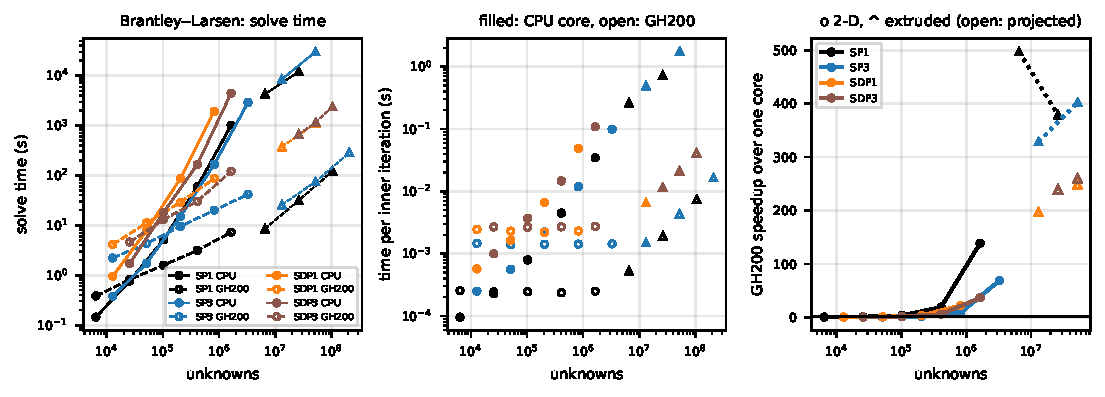
\includegraphics[width=0.95\textwidth]{perf_bl.pdf}
\caption{Brantley--Larsen, Marshak vacuum, on identical meshes: solve time
(left), time per inner iteration (middle) and the GH200's speedup over one
CPU core (right). CPU filled markers and solid lines, GH200 open markers and
dashed lines; circles 2-D meshes, triangles extruded ones. In the right
panel, open triangles are speedups with a projected one-core time
(Table~\ref{tab:perf-proj}).}
\label{fig:perf-bl}
\end{figure}

\begin{table}[h]
\caption{Brantley--Larsen solve times on identical $n \times n$ meshes. CPU:
best of three on one core, or a single solve ($^1$) where one takes hours.
GH200: best of three, single solves for the largest extruded cases. Extruded
rows ($n_z > 1$) follow the 2-D ones. Iteration counts are the GH200 run's;
GH200 GB is the memory CuPy's pool held after the solve; $|\Delta k|$ is the
CPU--GPU difference. OOM: out of GH200 memory; cap: an inner solve hit its
5000-iteration cap; cancelled: stopped on purpose; --: not run. One-core
projections for the extruded GMRES cases are in Table~\ref{tab:perf-proj}.}
\label{tab:perf-bl}
\tablefile{perf_bl}
\end{table}

\begin{figure}[h]
\centering
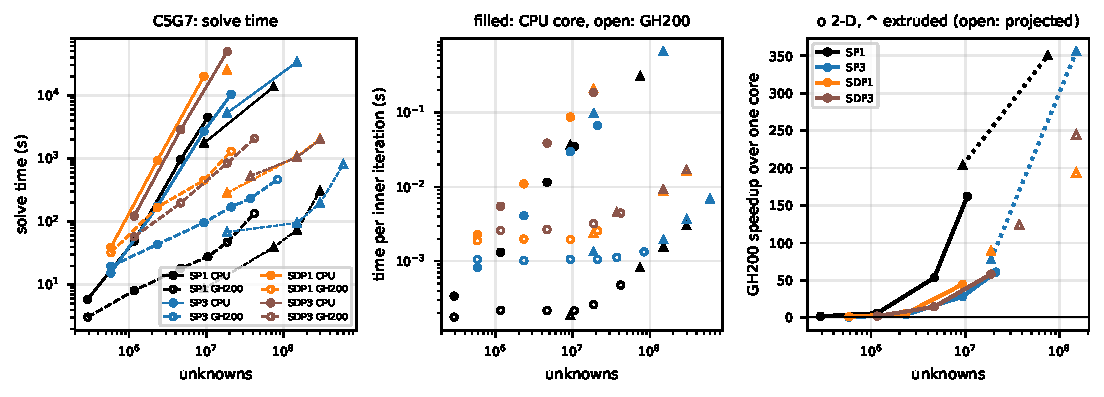
\includegraphics[width=0.95\textwidth]{perf_c5g7.pdf}
\caption{C5G7 pin-resolved, Marshak vacuum: as Fig.~\ref{fig:perf-bl}.}
\label{fig:perf-c5g7}
\end{figure}

\begin{table}[h]
\caption{C5G7 pin-resolved solve times on identical meshes ($s$ cells per pin
side); as Table~\ref{tab:perf-bl}.}
\label{tab:perf-c5g7}
\tablefile{perf_c5g7}
\end{table}

\begin{table}[h]
\caption{Projected one-core times of the extruded GMRES cases without a
converged CPU run (status of 2 November 2026). CPU run: what happened to the
one-core run (cap: stopped at the 5000-iteration cap; cancelled: stopped on
purpose; running). ns: one core's time per inner iteration per cell-moment
in the basis run; ``(cap)'' marks a basis timed from a cap run's log.
Projected CPU time = ns $\times$ cell-moments $\times$ GH200 inners;
uncertainty about $\pm 25$\%.}
\label{tab:perf-proj}
\tablefile{perf_projection}
\end{table}

\subsection{Results}

\textbf{Same answer on both devices.} Wherever both devices converged, they
give the same $k$ within $3 \times 10^{-10}$ on Brantley--Larsen. On C5G7 the
two runs can stop a few outer iterations apart and differ by up to
$7 \times 10^{-9}$, inside the $2 \times 10^{-8}$ allowed between equivalent
configurations. The extruded cases give the $k$ of the 2-D mesh they repeat
within $5 \times 10^{-9}$.

\textbf{Crossover.} On Brantley--Larsen the GH200 is faster than one core
from 0.1--0.2 million unknowns: $n = 160$ for SDP3 and $n = 320$ for the
other methods, where the CPU solve takes 5--90~s. On C5G7 it is faster from
the coarsest mesh, $s = 4$ (0.3--1.2 million unknowns), for every method
except SP3, which crosses at $s = 8$. Below the crossover the GH200 is up to
six times slower, because its fixed cost per iteration (below) dominates.

\textbf{Speedup on the largest meshes both devices ran}
(Tables~\ref{tab:perf-bl} and~\ref{tab:perf-c5g7}):

\begin{center}
\begin{tabular}{lrrrr}
\hline
 & SP1 & SP3 & SDP1 & SDP3 \\
\hline
Brantley--Larsen & 138 ($n = 1280$) & 69 ($n = 1280$) & 22 ($n = 640$) & 37 ($n = 640$) \\
C5G7             & 162 ($s = 24$)   & 61 ($s = 24$)   & 45 ($s = 16$)  & 58 ($s = 16$) \\
\hline
\end{tabular}
\end{center}

\noindent On these meshes one core takes 17~minutes (Brantley--Larsen SP1)
to 13.7~hours (C5G7 SDP3), and the GH200 7~s to 14~minutes. On every ladder
the speedup is still rising at the last mesh.

\textbf{Why the speedup grows} (middle panels of Figs.~\ref{fig:perf-bl}
and~\ref{fig:perf-c5g7}). The cost of one inner iteration behaves differently
on the two devices.
\begin{itemize}
\item \emph{GH200.} The time per inner iteration is constant up to a few
  million cell-moments: 0.18--0.25~ms for SP1, 1.0--1.4~ms for SP3,
  1.9--2.6~ms for SDP1 and 2.6--3.2~ms for SDP3. In this regime the solve
  time depends only on the iteration count, not on the mesh. Above it the
  time grows linearly with the mesh. On the largest meshes it is
  0.07--0.08~ns per cell-moment per iteration for the CG methods (SP1, SP3)
  and 0.38--0.41~ns for the GMRES methods (SDP1, SDP3), whose iterations
  also orthogonalize against the stored Krylov basis.
\item \emph{CPU core.} The time grows linearly from the start, at 8--12~ns per
  cell-moment per iteration for SP1 and SP3 while a group's vectors fit in
  cache. It rises two- to threefold, to 21--30~ns, on the largest 2-D
  meshes; for SDP1 and SDP3 it goes from 27--36~ns to 60--70~ns.
\end{itemize}
Once both devices are in their linear regimes, the speedup tends to the ratio
of these per-unknown costs. The 2-D costs give about 280--380 for the CG
methods and 150--180 for GMRES. On the extruded meshes one core is slower per
unknown than on the largest 2-D meshes, so the speedups there come out
higher: 350--400 measured for CG and about 200--260 projected for GMRES
(below). Part of the largest speedups comes from the CPU working set leaving
the cache, which is what a realistic 3-D problem does on a CPU too.

\textbf{SP3 has a high fixed cost on the GH200.} SP3's time per iteration at
small sizes (1.0--1.4~ms) is five to six times SP1's, although its block has
only twice the unknowns. On the largest meshes the ratio falls to 2.2 (BL
with 256 layers: 16.6 against 7.4~ms per iteration), as the extra unknowns
predict. The extra fixed cost is per operator apply. The likely source is the
coupled Marshak term: \code{\_apply\_marshak} in \code{garnet/spn.py} applies
it as gathers, a batched $2 \times 2$ product and scatters over the boundary
cells, each a separate small kernel. This has not been profiled. If SP3's
fixed cost were twice SP1's, mid-sized SP3 solves on the GPU would be up to
about three times faster. It does not affect the CPU or the results.

\textbf{3-D-sized problems on one GH200.} The extruded cases reach the cell
counts of a 3-D core. They need 15--58\% more inner iterations than the 2-D
mesh they repeat, and the number does not grow with the layer count. A 2-D
ladder, by contrast, doubles its inner iterations with each mesh doubling.
The largest cases solved:
\begin{itemize}
\item Brantley--Larsen with 256 layers (105 million cells): SP1 in 122~s
  and SP3 (210 million unknowns) in 287~s.
\item C5G7 at $s = 16$ with 64 layers (42.6 million cells, 7 groups): SP1
  (298 million unknowns) in 306~s and SP3 (597 million) in 807~s, using
  77~GB.
\item C5G7 at $s = 8$: SDP1 with 128 layers and SDP3 with 64 layers (298
  million unknowns each) in 2040 and 1990~s.
\end{itemize}
After the solve, CuPy's memory pool held 130--250 bytes per unknown on the
extruded C5G7 cases (SP3 lowest, about 210--220 for SDP1 and SDP3), and
260--510 on the one-group Brantley--Larsen problem, where per-cell data is
shared by fewer unknowns. Two cases ran out of the GH200's 96~GiB (102.6~GB),
both at 597 million unknowns: SDP1 at $s = 16$ with 64 layers and SDP3 at
$s = 8$ with 128. Both stopped in the first GMRES solve with 100.6~GB
allocated, of which the 61-vector Krylov basis alone is 42~GB. By these
figures, one GH200 holds a 7-group 3-D problem of roughly 450 million
unknowns with SDP1 or SDP3, and 400--800 million with SP1 or SP3.

\textbf{Extruded cases on one core.} The CPU runs covered all four methods
at 16 and 64 layers of Brantley--Larsen and at 8 and 64 layers of C5G7 at
$s = 8$, with SDP3 at 32 layers instead of 64: at 64 layers it would take
110--140~h on one core, beyond the 5-day job limit, so the GH200 also ran
SDP3 at 32 layers for the comparison.
\begin{itemize}
\item \emph{Measured:} SP1 and SP3 at every extruded size, and C5G7 SDP1 at
  8 layers. With 64 layers the GH200 is 350--400 times faster than one core:
  379 (SP1) and 402 (SP3) on Brantley--Larsen, 350 and 355 on C5G7. Where
  the GH200 is still in its fixed-cost regime the speedup is lower: 77 for
  C5G7 SP3 and 89 for C5G7 SDP1, both at 8 layers. On the extruded meshes
  one core takes 28--37~ns per cell-moment per iteration for SP1 and SP3,
  somewhat more than on the largest 2-D meshes, and 79~ns for C5G7 SDP1.
  Brantley--Larsen SP1 at 16 layers took 39~ns, 40\% more than at 64 layers,
  which gives it a speedup of 498. Whether contention with the other runs
  inflated it will show in the alone re-run at the end of the job.
\item \emph{Failed at the iteration cap:} Brantley--Larsen SDP1 at 16 layers
  and SDP3 at 32 layers, although the GH200 converged on the same meshes.
  Both stopped in the first outer iteration at the 5000-iteration cap, with
  residuals 1.45 and 1.6 times the target. The CPU orthogonalizes the Krylov
  basis by modified Gram--Schmidt and the GH200 by two-pass classical
  Gram--Schmidt. At these sizes the Jacobi-preconditioned GMRES is so close
  to the cap that this rounding difference decides the outcome (finding~5).
\item \emph{Stopped on purpose:} Brantley--Larsen SDP1 at 64 layers and C5G7
  SDP1 at 64 layers and SDP3 at 32 layers, after 4--11~h of an expected
  60--80~h each. They would have added more GMRES points of the kind the
  projections below already estimate.
\item \emph{Still running} (2 November): Brantley--Larsen SDP3 at 16 layers
  and C5G7 SDP3 at 8 layers.
\end{itemize}

\textbf{Projected GMRES speedups} (Table~\ref{tab:perf-proj}, open
triangles in the right panels of Figs.~\ref{fig:perf-bl}
and~\ref{fig:perf-c5g7}). For an extruded GMRES case without a converged CPU
run, the one-core time is projected from three numbers:
\begin{itemize}
\item one core's measured time per inner iteration per cell-moment in a
  basis run;
\item the case's number of cell-moments;
\item the GH200's inner iteration count for the case.
\end{itemize}
The two cap runs give the basis at large sizes: their 5000 iterations,
timed from their logs, took 98~ns (SDP1, 16 layers) and 105~ns (SDP3, 32
layers) per cell-moment. C5G7 SDP1 at 8 layers (79~ns, converged) gives the
basis for C5G7 SDP1. C5G7 SDP3 has no measurement yet and borrows the
Brantley--Larsen SDP3 cost. The projected speedups are 194--260 at 13--149
million unknowns, and 124 for C5G7 SDP3 at 8 layers, where the GH200 is
still near its fixed-cost regime. Three sources of uncertainty add up to
about $\pm 25$\%:
\begin{itemize}
\item the CPU and GH200 inner iteration counts of converged runs differ by
  up to 7\%;
\item the cap runs' iterations are full restart cycles of a first outer
  iteration, which may cost slightly more per iteration than the average;
\item a cost carried over from another mesh or problem adds the spread seen
  between measured per-cell costs (79--105~ns for GMRES).
\end{itemize}
At 3-D sizes the GH200 is therefore about 200--260 times faster than one
core for SDP1 and SDP3 (projected), against 350--400 times for SP1 and SP3
(measured): GMRES's orthogonalization takes a larger share of the GH200's
time than of the CPU's.

\textbf{Concurrency control.} Re-timed alone after the concurrent runs had
finished, Brantley--Larsen SP3 at $n = 640$ took 166.3~s against 167.3~s
side by side (0.6\%), and C5G7 SP3 at $s = 8$ took 169.0~s against 174.8~s
(3.4\%). Running the methods side by side inflates the 2-D CPU times by a
few percent at most, and the speedups by the same amount. The extruded jobs
each end with a similar control (Brantley--Larsen SP1 at 16 layers and C5G7
SP1 at 8 layers, re-timed alone), still pending on 2 November.

\textbf{FEMFFUSION, for scale.} The paper reports 1.1--2.6~s for
Brantley--Larsen with FEMFFUSION, using second-degree elements on an
$80 \times 80$ mesh (about 26\,000 nodes per moment) on unstated hardware.
Its $k$ values agree with \garnet's mesh limits within 0.6~pcm
(Section~\ref{sec:bl}). \garnet's finite volumes reach a comparable mesh
error (about 2~pcm) at $n = 640$, where one core takes 60--4400~s and the
GH200 3--121~s. At this problem size a higher-order discretization does
better than a faster device. The GH200 pays off at the sizes of a 3-D core,
where any discretization has tens to hundreds of millions of unknowns.

